%%%%%%%%%%%%%%%%%%%%%%%%%%%%%%%%%%%%%%%%%%%%%%%%%%%%%%%%%%%%%%%%%%%%%%%%%%%%%%%%
\documentclass[twocolumn]{revtex4}

%%%%%%%%%%%%%%%%%%%%%%%%%%%%%%%%%%%%%%%%%%%%%%%%%%%%%%%%%%%%%%%%%%%%%%%%%%%%%%%%
% Note that comments begin with a "%" and are not turned into text in the .pdf
% document.
%%%%%%%%%%%%%%%%%%%%%%%%%%%%%%%%%%%%%%%%%%%%%%%%%%%%%%%%%%%%%%%%%%%%%%%%%%%%%%%%

%%%%%%%%%%%%%%%%%%%%%%%%%%%%%%%%%%%%%%%%%%%%%%%%%%%%%%%%%%%%%%%%%%%%%%%%%%%%%%%%
% Include some extra packages.
%%%%%%%%%%%%%%%%%%%%%%%%%%%%%%%%%%%%%%%%%%%%%%%%%%%%%%%%%%%%%%%%%%%%%%%%%%%%%%%%
\usepackage[]{graphicx}
%%%%%%%%%%%%%%%%%%%%%%%%%%%%%%%%%%%%%%%%%%%%%%%%%%%%%%%%%%%%%%%%%%%%%%%%%%%%%%%%

%%%%%%%%%%%%%%%%%%%%%%%%%%%%%%%%%%%%%%%%%%%%%%%%%%%%%%%%%%%%%%%%%%%%%%%%%%%%%%%%
\begin{document}

%%%%%%%%%%%%%%%%%%%%%%%%%%%%%%%%%%%%%%%%%%%%%%%%%%%%%%%%%%%%%%%%%%%%%%%%%%%%%%%%
\title{
Journal article
}

\author{S.~Tibbitts}
\affiliation{Siena College, Loudonville, NY}

\date{\today}

\begin{abstract}
    This project came about as the assignment for my CSIS 200 final project.  The goal of the project was to come up with a way to predict the rainfall for each month with pre-written conditions.  By using python, I was able to determine the chance it rains once a month, 8 or more times per month, at least 10 cms per month, the average rainfall per month, and a distribution of the rainfall.  While there is a very low chance it only rains once a month or 8-plus days, over $\frac{3}{10}$ months will have at least 10 cm of rain, and on average it will rain approximately 8 cm per month.
\end{abstract}

\maketitle
%%%%%%%%%%%%%%%%%%%%%%%%%%%%%%%%%%%%%%%%%%%%%%%%%%%%%%%%%%%%%%%%%%%%%%%%%%%%%%%%

%%%%%%%%%%%%%%%%%%%%%%%%%%%%%%%%%%%%%%%%%%%%%%%%%%%%%%%%%%%%%%%%%%%%%%%%%%%%%%%%
\section{Introduction}

The motivation behind this project came from Dr. Bellis, who assigned this as my final project.  The project was designed to incorporate everything that we had learned throughout the year in python into a practical application.  The overall goal of the project was to come up with code to determine how often it rains a certain number/range of days per month, as well as the amount of rainfall per month.
%%%%%%%%%%%%%%%%%%%%%%%%%%%%%%%%%%%%%%%%%%%%%%%%%%%%%%%%%%%%%%%%%%%%%%%%%%%%%%%%


%%%%%%%%%%%%%%%%%%%%%%%%%%%%%%%%%%%%%%%%%%%%%%%%%%%%%%%%%%%%%%%%%%%%%%%%%%%%%%%%
\section{Question 1}
"Suppose there is a 20\% chance it will rain on any given day in a month.  What are the odds that it rains on one and only one day in a month?"
To work out this problem, you have to take into account that it can rain on \textbf{ANY} day in the month, not just one specific day.  To account for this, you have to take the probability that the day it rains on will be the first day \textbf{OR} the second day \textbf{OR} the third day, and so on.  The formula would look something like this: 
$$ ( \frac{20}{100}_1 + \frac{20}{100}_2 + \frac{20}{100}_3 .... + \frac {20}{100} _ {30} ) \times (\frac{80}{100})^{29} \times 100 = 0.928 \%$$

The sumation of fractions represents how the one day of rain can be anyday of the month, and the sum is multiplied by $(\frac{80}{100}) ^{29} $ because no matter what day it rains on, the other 29 days will not rain.


To approach this problem numerically in python, I created a function that goes through a random set of days and tests whether or not it rains only one day that month.  In the function, I set the chance of rain equal to 20 percent, and created a loop in which every day in the month is tested to determine whether or not it will rain that day. If a day tested does in fact pass this test, a counter will increase by one.  Since we only care whether or not it rains only one day per month, if the counter's value is greater that 1, the loop will break and the function will return as \textbf{False.}  Also, if the function determines that there are no days of rain in the entire month, it will return as \textbf{False}.  To obtain a numerical value for the percentage of months it rains only once, we need to run this function over and over again.  By creating a loop that loops over our created function a certain amount of times, I came up with an accurate answer.  The more times the function is looped over, the more accurate the figure achieved will be.  In this loop, a new set of days will be generated for each trial tested.  If said trial returns as \textbf{True}, the counter will increase by 1.  To obtain the percentage figure, I used the following formula: $ \frac{counter}{total months} * 100 \approx 0.92 \% $. 

\section{Question 2}

This scenario can be tested very similaly to the first one.   Similar to the problem in the first scenario, I created a function to test how many days in a month it rains.  In the funcition, I created a variable and set the chance of rain equal to 0.10, and test to see whether or not it rains 8 or more days in the month.  To do this, I ran a loop through the days of the month, and if a day's value falls under the chance of rain, the counter increases by 1.  If the counter reaches 8, the loop will break and the function will return \textbf{True}.  Otherwise, the function returns \textbf{False}.  To obtain a percentage for how often it rains 8 or more days per month, we will loop over this funciton with new sets of random days like in the first example.  The percentage given is equal to $ \frac{raincounter}{nmonths} * 100 \approx  0.70 \% $

\section{Question 3}



\subsection{3a} 

In order to find the chance it rains at least \textbf{10 cm} in a month, we must create a new function that takes in a month's worth of days.   In the function, the chance it rains depends on if it rained the day beforehand.  To make sure this was taken into account for, I created a set of conditionals.  If the day in the month satisfies a conditional, that day is given a value of \textbf{True}.  Everytime a value is deemed to be true, a counter increases by \textbf{1}.  In order to determine how much it rains in the month, another set of conditionals is needed.  These conditionals will be looped over $x$ amount of times, where $x$ is equal to the number of days it rains in each month.  For each day, a random number will be generated, and depending on the range this number falls within, it will rain a certain number of centimeters.  The amount of rain each day is added to a new counter, and this counter is returned by the function.  To obtain a percentage of months it rains at least \textbf{10 cm}, I looped over this function $n$ amount of times.  In the loop, a new month is generated each time the function is looped over.  A conditional then tests if the month did in fact have \textbf{10 cm} of rain.  If it did, the counter increases by \textbf{1}.  The percentage of months it rains \textbf{10 cm} is then equal to $ \frac{10cm~Months}{nmonths} * 100 \approx 34 \% $.

\subsection{3b}

To create a histogram to show the distribution of rainfall, I am able to use the values from all of the months tested in \textit{3a}.  In the final loop used to obtain the percentage, I appended all of the values to a list, so they could be stored for the histogram.   To create the figure, I set the figure size to (5,5).  Then, I plot the histogram by giving the command the list of values, the number of bins, and the range that the bins span over.  I then labeled the x - axis and y - axis accordingly.

\begin{figure}[h]
\centering

\caption{Note that the low edge of the bin represents the amount of rain per month.}

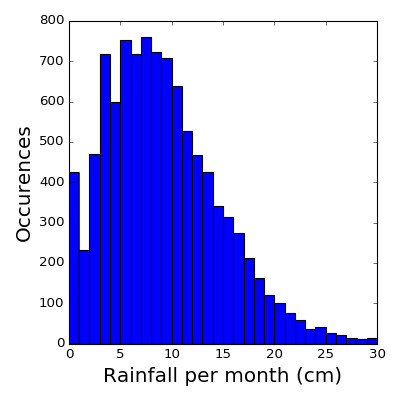
\includegraphics[width = 0.35\textwidth]{histogram.png}

\end{figure}

\subsection{3c}

To calculate the aberage rainfall per month, I looped over the list of values obtained in \textit{3a}.  I add the value of rain in each individual month out of the list, and divide by the total number of months tested in the list.  The average rainfall per month is $ \frac{total~ rain}{nmonths} \approx 8$~cm per month.

\subsection{3d}

In order to determine a range to quote, I sorted the list of values obtained in \textit{3a} so that they were listed in numerical order.  From there, I can take the range from the 2.5\% position to the 97.5\% postion.  I'm 95 \% confident that the rainfall will be between 0 and 19 cm per month.

%%%%%%%%%%%%%%%%%%%%%%%%%%%%%%%%%%%%%%%%%%%%%%%%%%%%%%%%%%%%%%%%%%%%%%%%%%%%%%%%

%%%%%%%%%%%%%%%%%%%%%%%%%%%%%%%%%%%%%%%%%%%%%%%%%%%%%%%%%%%%%%%%%%%%%%%%%%%%%%%%
\end{document}
%%%%%%%%%%%%%%%%%%%%%%%%%%%%%%%%%%%%%%%%%%%%%%%%%%%%%%%%%%%%%%%%%%%%%%%%%%%%%%%%
